\section{CONCLUSION}
\label{S:conclusion}

We present two algorithms based on trees and random forests for receding horizon control with data-driven models.

We compare the performance of our Data Predictive Control to MPC on a multivariable bilinear building model. We establish that DPC with random forests shows a remarkable similarity to MPC in the optimal control strategies explaining $70\%$ variance. On the other hand, DPC with regression trees suffers from practical limitations due to model overfitting.

We further apply DPC with random forests to a large scale 6 story EnergyPlus model with 22 zones for which the traditional model-based control is largely unsuitable due to complex dynamics and the cost of model identification. We show that DPC, relying only on the sensor data, can provide significant energy savings while maintaining thermal comfort. Our results demonstrate that even for such complex system, DPC tracks a reference signal with a mean error of $3\%$.

\begin{figure}[t!]
	\begin{center}
		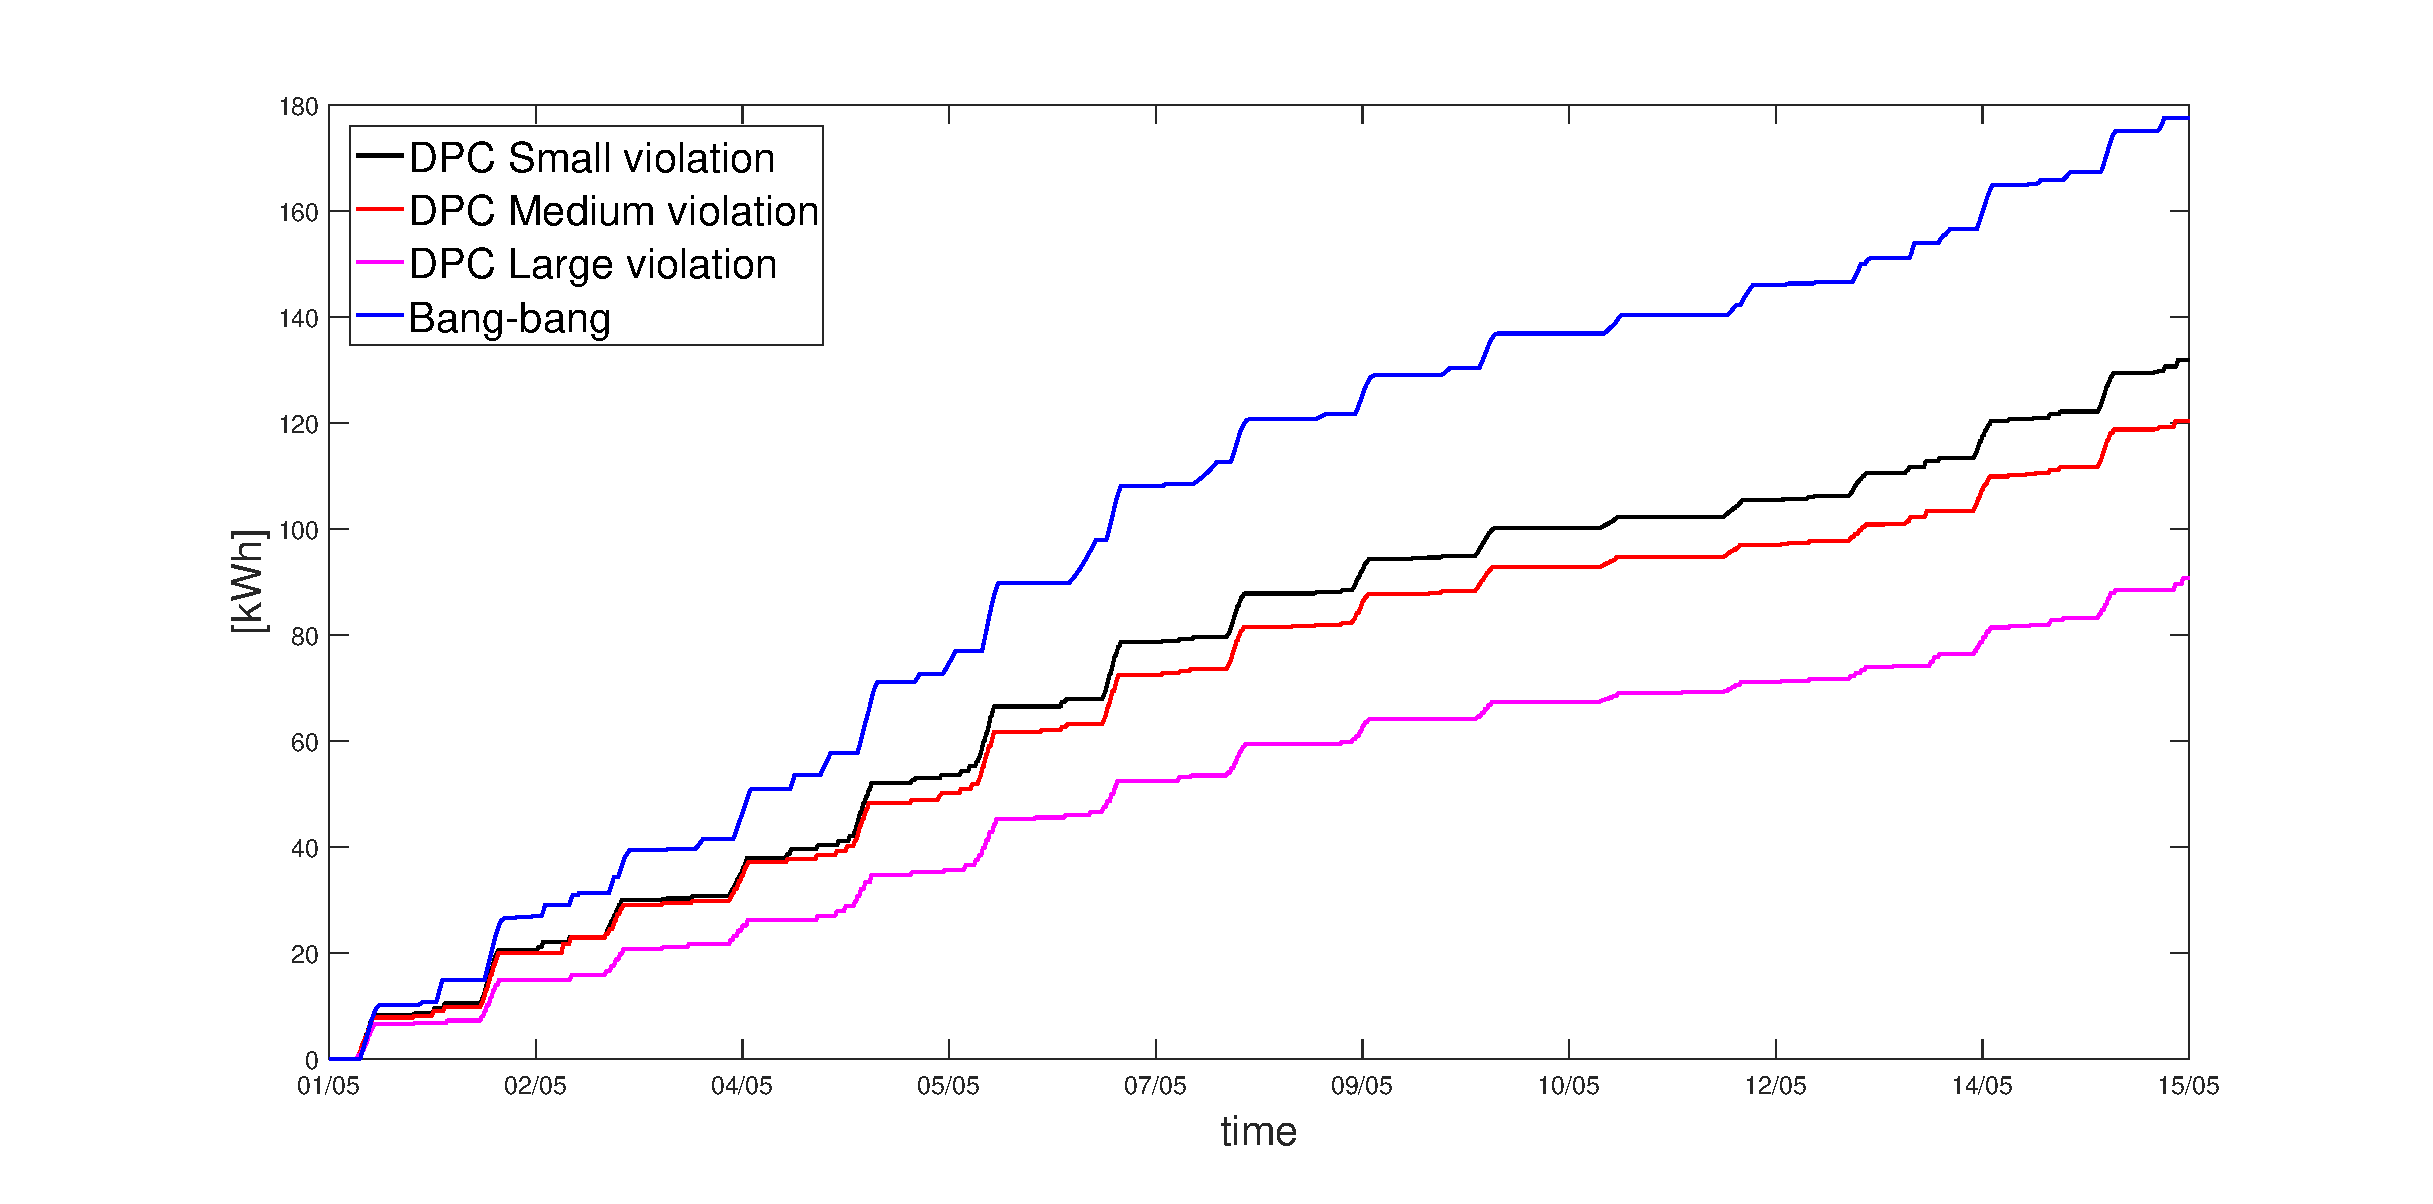
\includegraphics[width=26pc]{figures/Energy_all_EnergyPlus.eps}
	\end{center}
	\caption{Comparison of DPC and bang-bang controller performance in terms of thermal energy saving with different violations using EnergyPlus model.}
	\label{F:comparison_all_energy_E+}
\end{figure}

We finally apply DPC using data from a real house and compare it with the classical bang-bang controller widely used for temperature control in houses. We implemented DPC to guarantee energy saving while guaranteeing thermal comfort for the occupants. We obtained, with respect to a bang-bang controller, an energy saving that goes from the $25.4\%$, when we want the temperature to be strictly in a comfort range, to the $49.2\%$, if we allow little violations of such a range.

DPC has applications which go beyond buildings and energy systems, to industrial process control, and controlling large critical infrastructures like water networks, district heating \& cooling. DPC is immensely valuable in situations where first principles based modeling cost is extremely high.

\subsection{Practical Challenges and Future Work}
\label{SS:challenges}
\textit{Data Availability:} The main practical challenge for DPC lies in the availability of data for training and we require answers to questions like how much data (functional testing) is required, and how should the sampling be done? Therefore, the procedure for optimal experiment design, and model improvement with estimation of variance in predictions is one of the main focus of our ongoing work.

\textit{Stability:} While the buildings are inherently stable, many other applications require stability guarantees. In our ongoing work, we are working towards proving asymptotic stability to origin with DPC-RT and DPC-En by using concept of switched LTI systems. This will make DPC useful for systems with faster dynamics.

\textit{Robustness:} Another direction of work is on handling uncertainties in the DPC framework, namely an extension to Scenario DPC to account for the disturbance uncertainty. This will help us in quantifying the robustness of DPC.
